\documentclass[../../main.tex]{subfiles}
\graphicspath{{\subfix{../../images/}}}


\begin{document}

\subsection{Architektura chmurowa}
    \subsubsection{Wstęp}
        Architektura chmurowa została napisana w oprogramowaniu HashiCorp Terraform i wdrożona na serwery Amazon Web Services (AWS)\cite{aws}. HashiCorp Terraform (albo krótko Terraform)\cite{terraform} to oprogramowanie Infrastructure as Code (IaC) pozwalające na skryptowe wdrażanie infarstruktury na serwery dostawcy.
    \subsubsection{Struktura plików}
        Struktura plików została podzielona ze względu na środowisko produkcyjne i testowe. Na Rysunku \ref{fig:aws-repo-structure} przedstawione jest tylko środowisko produkcyjne ze względu na tą samą strukturę systemu plików. Z tego samego względu omówione zostanie tylko środowisko produkcyjne.
        
        \begin{figure}[ht!]
            \centering
            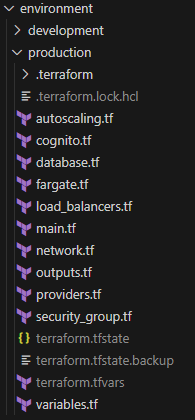
\includegraphics[height=0.4\pdfpageheight]{images/aws-repo-structure.png}
            \caption{Struktura plików Terraform}
            \label{fig:aws-repo-structure}
        \end{figure}

        Pliki .tf zawierają opis zasobów wdrażanych na serwery. Plik .tfstate przechowuje dokładny spis zasobów już wdrożonych wraz z ich unikalnymi identyfikatorami, sekretami, itd. Opis pozostałych plików:
        \begin{itemize}
            \item main.tf - wersje oprogramowania wykorzystywane w projekcie
            \item providers.tf - konfiguracja dostawcy AWS
            \item variables.tf - spis wszystkich zmiennych wraz z ich opisami i niektórymi wartościami domyślnymi
            \item terraform.tfvars - niewersjonowany plik zawierający wartości niektórych zmiennych; przede wszystkim przechowuje sekrety
            \item outputs.tf - zbiór przydatnych wartości wyjściowych, np. nazwa DNS Application Load Balancera
            \item network.tf - zasoby sieciowe: VPC, brama sieciowa, tablice routingu, podsieci
            \item security\_groups.tf - grupy bezpieczeństwa (działają jak zapora ogniowa) konfigurujące przychodzący i wychodzący ruch sieciowy
            \item cognito.tf - dostawca tożsamości Amazon Cognito i jego konfiguracja
            \item load\_balancers.tf - Application Load Balancer, zasoby nasłuchujące na portach 80, 443 i 8080 oraz grupy celów
            \item fargate.tf - definicje zadań wykonywanych przy pomocy AWS Fargate oraz serwisy które nimi zarządzają
            \item autoscaling.tf - zestaw reguł pozwalających na automatyczne zmniejszanie lub zwiększanie liczby działających instancji modułów (frontendu i backendu)
            \item database.tf - konfiguracja bazy danych RDS
        \end{itemize}
    \subsubsection{Wykorzystane zasoby}
        \begin{itemize}
            \item \textbf{Amazon Virtual Private Cloud (VPC)}
            \item \textbf{Amazon Cognito}
            \item \textbf{Amazon Relational Database Service (RDS)}
            \item \textbf{Amazon Application Load Balancer (ALB)}
            \item \textbf{Amazon Elastic Container Service (ECS)}
            \item \textbf{Amazon Certificate Manager (ACM)}
            \item \textbf{Amazon CloudWatch}
            \item \textbf{Amazon Simple Storage Service (S3)}
            \item \textbf{AWS Auto Scaling}
        \end{itemize}

\end{document}